% The document class supplies options to control rendering of some standard
% features in the result.  The goal is for uniform style, so some attention 
% to detail is *vital* with all fields.  Each field (i.e., text inside the
% curly braces below, so the MEng text inside {MEng} for instance) should 
% take into account the following:
%
% - author name       should be formatted as "FirstName LastName"
%   (not "Initial LastName" for example),
% - supervisor name   should be formatted as "Title FirstName LastName"
%   (where Title is "Dr." or "Prof." for example),
% - degree programme  should be "BSc", "MEng", "MSci", "MSc" or "PhD",
% - dissertation title should be correctly capitalised (plus you can have
%   an optional sub-title if appropriate, or leave this field blank),
% - dissertation type should be formatted as one of the following:
%   * for the MEng degree programme either "enterprise" or "research" to
%     reflect the stream,
%   * for the MSc  degree programme "$X/Y/Z$" for a project deemed to be
%     X%, Y% and Z% of type I, II and III.
% - year              should be formatted as a 4-digit year of submission
%   (so 2014 rather than the accademic year, say 2013/14 say).

\documentclass[ % the name of the author
                    author={Ashwinder Khurana},
                % the name of the supervisor
                supervisor={Prof Dave Cliff},
                % the degree programme
                    degree={MEng},
                % the dissertation    title (which cannot be blank)
                     title={The Deeply Reinforced Trader},
                % the dissertation subtitle (which can    be blank)
                  subtitle={},
                % the dissertation     type
                      type={enterprise},
                % the year of submission
                      year={2020} ]{dissertation}
                      
                      
\usepackage{float} 
\usepackage{subfig}

\begin{document}

% =============================================================================

% This section simply introduces the structural guidelines.  It can clearly
% be deleted (or commented out) if you use the file as a template for your
% own dissertation: everything following it is in the correct order to use 
% as is.



% =============================================================================

% This macro creates the standard UoB title page by using information drawn
% from the document class (meaning it is vital you select the correct degree 
% title and so on).

\maketitle

% After the title page (which is a special case in that it is not numbered)
% comes the front matter or preliminaries; this macro signals the start of
% such content, meaning the pages are numbered with Roman numerals.

\frontmatter

% This macro creates the standard UoB declaration; on the printed hard-copy,
% this must be physically signed by the author in the space indicated.

\makedecl

% LaTeX automatically generates a table of contents, plus associated lists 
% of figures, tables and algorithms.  The former is a compulsory part of the
% dissertation, but if you do not require the latter they can be suppressed
% by simply commenting out the associated macro.

\tableofcontents
\listoffigures
\listoftables
\listofalgorithms
\lstlistoflistings

% The following sections are part of the front matter, but are not generated
% automatically by LaTeX; the use of \chapter* means they are not numbered.

% -----------------------------------------------------------------------------

\chapter*{Executive Summary}

\noindent
One of the primary goals of artificial intelligence is the solve complex tasks that rely on highly dimensional, unprocessed and noisy input. Namely, recent advances in Deep Reinforcement Learning (DRL) has resulted in the "Deep Q Network \cite{DQN}, which is capable of human level performance on several Atari video games - using unprocessed pixels for input. A similar "gamification" of the process of a continuous double auction limit-order-book (LOB), can be an application of DRL.
\\
\\
DRL requires for an agent to interact with an environment and to derive actions from the state of the environment at each timestep. The environment in this case can be a market session, in which several sales traders interact and utilise the LOB to communicate orders to buy or sell an asset, and the agent that interacts with the environment is the proprietary trader, which aims to seek profit for itself rather than on the behalf of a client. Information available from the LOB can be used as combinations of inputs to represent the current state of the 'game', from which the trader can learn which actions to take during the learning process. This is done by using a policy which determines what action to take depending on the current state of the LOB and a reward system which provides rewards depending on the action.
\\
Falcao had used a Policy Gradient agent (PG Agent) in conjunction with Cliff's ZIP to solve the sales trader problem. In comparison this thesis attempts to solely use state of the art DRL techniques to solve the proprietary trader problem, namely via models such as Advantage Actor-Critic, Policy Gradient and DDPG. 
\\
\\
Whilst most algorithms are trained and analysed with data from public exchanges collected from sites such as finance.yahoo.com, this thesis focuses on using Cliff's Bristol Stock Exchange \cite{BSE} and Falcao's Bristol Stock Gym \cite{BSG} to simulate market sessions of robot traders to train and compare the effectiveness of the agent against other traditional machine learning based algorithms.
\\
\\
This is a hugely challenging task as the mapping between the current state of the system and the action the agent takes in such an environment is a problem all financial institutions are aiming to tackle in the most sophisticated ways to gain an overall competitive advantage. The results of this thesis are not a success story, but it details the journey of iterating and analysing results to create a profitable trader using the techniques outlined above and the vast challenges that were presented.   

\begin{quote}
My research hypothesis is that the latest developments in machine learning, more specifically, a trader that uses Deep Reinforcement Learning techniques alone provide a tool set to create a proprietary trader that outperforms humans.  
\end{quote}

\noindent
This project explores the hypothesis 


\begin{quote}
\noindent
\begin{itemize}
\item I spent $100+$ hours researching prior work on the field and learning about Deep Reinforcement Learning techniques. 
\item I wrote a total of $\color{red}{?}$ lines of source code, comprising of the merger of capabilities of BSE into Falcao's BristolStockGym, several DRL models, Variational Auto-Encoder and Regression Models.
\item Spent $100+$ hours training the various models and running experiments on Blue Crystal 4 \cite{BC4} 
\end{itemize}
\end{quote}

% -----------------------------------------------------------------------------

\chapter*{Supporting Technologies}

\begin{quote}
\noindent
\begin{itemize}
\item All the codebase is written using Python version 3.6.7 and the Python Package Installer PIP tool in its 19.0.3 version.
\item Several Python libraries were used extensively throughout the project, namely: PyTorch(1.3.0), NumPy(1.18.1), Matplotlib(3.1.3), Sklearn(0.22)
\item I used a Falcao's version of Cliff's Bristol Stock Exchange that is refactored to be compatible for Deep Reinforcement Learning analogous to OpenAI's Gym 

\end{itemize}
\end{quote}

% -----------------------------------------------------------------------------

\chapter*{Notation and Acronyms}

\noindent
All of the acronyms used in this document are explained on their first usage and no more. However, several acronyms are used across multiple chapters throughout the thesis, they are as follows:

\section*{Acronyms}

\begin{quote}
\noindent
\begin{tabular}{lcl}
AI         &:     & Artificial Intelligence                         \\
BSE     &:     & Bristol Stock Exchange                     \\
BSG    &:      & Bristol Stock Gym                              \\
LOB    &:     & Limit Order Book                                \\
CDA    &:     & Continuous Double Auction                \\
MDP   &:      & Markov Decision Process                  \\
DRL     &:     & Deep Reinforcement Learning           \\
PG      &:      & Policy Gradient                                   \\
DDPG &:      & Deep Deterministic Policy Gradient    \\
ZI-C    &:       & Zero Intelligence - Constrained          \\
ZIP     &:      & Zero Intelligence Plus                          \\
DRT   &:      & Deeply Reinforced Trader                    \\


                    &\vdots&                                                                      \\
${\mathcal H}( x )$ &:     & the Hamming weight of $x$                                            \\
${\mathbb  F}_q$    &:     & a finite field with $q$ elements                                     \\
$x_i$               &:     & the $i$-th bit of some binary sequence $x$, st. $x_i \in \{ 0, 1 \}$ \\
\end{tabular}
\end{quote}

% -----------------------------------------------------------------------------

\chapter*{Acknowledgements}

{\bf An optional section, of at most $1$ page}
\vspace{1cm} 

\noindent
It is common practice (although totally optional) to acknowledge any
third-party advice, contribution or influence you have found useful
during your work.  Examples include support from friends or family, 
the input of your Supervisor and/or Advisor, external organisations 
or persons who  have supplied resources of some kind (e.g., funding, 
advice or time), and so on.

% =============================================================================

% After the front matter comes a number of chapters; under each chapter,
% sections, subsections and even subsubsections are permissible.  The
% pages in this part are numbered with Arabic numerals.  Note that:
%
% - A reference point can be marked using \label{XXX}, and then later
%   referred to via \ref{XXX}; for example Chapter\ref{chap:context}.
% - The chapters are presented here in one file; this can become hard
%   to manage.  An alternative is to save the content in seprate files
%   the use \input{XXX} to import it, which acts like the #include
%   directive in C.

\mainmatter

% -----------------------------------------------------------------------------

\chapter{Contextual Background}
\label{chap:context}

%This chapter should describe the project context, and motivate each of
%the proposed aims and objectives.  Ideally, it is written at a fairly 
%high-level, and easily understood by a reader who is technically 
%competent but not an expert in the topic itself.
%
%In short, the goal is to answer three questions for the reader.  First, 
%what is the project topic, or problem being investigated?  Second, why 
%is the topic important, or rather why should the reader care about it?  
%For example, why there is a need for this project (e.g., lack of similar 
%software or deficiency in existing software), who will benefit from the 
%project and in what way (e.g., end-users, or software developers) what 
%work does the project build on and why is the selected approach either
%important and/or interesting (e.g., fills a gap in literature, applies
%results from another field to a new problem).  Finally, what are the 
%central challenges involved and why are they significant? 
% 
%The chapter should conclude with a concise bullet point list that 
%summarises the aims and objectives.  For example:

\section{Introduction}

The underlying context behind this thesis is the comprehension, analysis and exploitation of the mechanisms that underpin the real-world financial markets, from a Computer Scientist's perspective. The infrastructure and mechanism of interest are major stock exchanges. Stock exchanges are where individuals or institutions come to a centralised market to buy and sell stocks, where the price of these stocks are set by the supply and demand in the market as the buyers and sellers place their orders on the exchange. There are various types of orders that can be used to trade a stock, however, this thesis focuses on a specific type of order, the Limit Order. A limit order is a type of order to purchase or sell a security at a specified price or better. For buy limit orders, the order will be executed only at the limit price or a lower one, while for sell limit orders, the order will be executed only at the limit price or a higher one \cite{limit-order}. 
A collection of orders of this kind formulates the Limit-Order-Book (LOB) , which is a book, maintained by the exchange, that records the outstanding limit orders made by traders.  
\\
\\
The role of a sales trader is to trade on behalf of a client, which means that they do not own a stock of their own, but instead buys and sells to secure the best price for their client. A proprietary trader, or a "prop" trader on the other hand buys and sells stocks on their own behalf with their own capital with the aim of seeking profitable returns. Both types of traders have to constantly adapt to the market conditions and react through the prices they quote for their orders. 
\\
\\
Originally, the job of trading was fulfilled by humans who reacted to the market conditions using their intuition and their knowledge of the financial markets, however the job was hit with a wave of automation after 2001, when IBM researchers published results that indicated that two algorithms (ZIP by Prof Dave Cliff and MGD, a modification of GD by Steven Gjerstad \& John Dickhaut) consistently outperformed humans in a experimental laboratory version of financial markets \cite{algorithmic-trading-wiki}. 
\\
\\
Since then, there has been relatively little research done in this field within academia, and subsequent solutions have built upon the traditional heuristic alongside 'old school' machine learning approaches. Considering the explosion of Deep Learning as a field in this last decade, this thesis attempts to explore the application of these state-of-the-art techniques, in particular Deep Reinforcement Learning, to the problem of the adaptive prop trader.

\section{History of Research}
\subsection{Experimental Economics to Algorithmic Trading}
\label{section:history}
Analysis of the sales trader problem can be seen as early as the 1960's in Vernon Smith's experiments at Purdue University, which led to the birth of the field of Experimental Economics and a Nobel Prize for Smith. 
\\
\\
Smith's motivation behind these experiments was to find empirical evidence for the credibility of basic microeconomic theory of Continuous Double Auction's (CDA's) to generate competitive equilibria \cite{MarketEquilibrium} . He formalised this experiment structure as a Double-oral-Auction in which he would a split a group of humans up into two subgroups: Buyers and Sellers. He gave each human a private limit price, where buyers would not buy above that price and sellers would not sell below that price. Prices quoted by the buyer's are known as the bid prices and the prices quoted by the sellers are known as the ask prices. The buyers and sellers would interact within small time based sessions, otherwise known as trading sessions.
\\
\\
After running repeated experiments of the trading sessions, Smith empirically demonstrated that the prices quoted by the traders demonstrated rapid equilibration, where the prices would converge to the theoretical 'best' price of an asset, despite a small number of traders used.
\\
\\
These sets of experiments were repeated by Gode and Sunder \cite{Gode and Sunder}  in the 1990's. Crucially however, the human traders that were the core of Smith's experiments were replaced with computer based algorithmic traders. Gode and Sunder introduced two types of \textit{zero-intelligence} algorithmic traders for CDA markets: Zero Intelligence - Unconstrained (ZI-U) and Zero Intelligence - Constrained (ZI-C). ZI-U traders are traders that generated a uniformly random bid/ask price, whilst ZI-C traders were traders that also generated a random price, however it was constrained between the private limit price of the trader and the lowest/highest possible price w.r.t to whether it was a buyer or seller - therefore it could never sell at a loss.
\\
\\
The purpose of Gode and Sunder replicating the experiments by Smith with their adaptation from humans to computers was to figure out if the {\color{red}allocative efficiency} of a market was down to the intelligence of the traders or the organisation of the market. They ran several experiments with 5 different types of market structures whilst monitoring their allocative efficiency. They concluded that the ZI-U traders were essentially useless in that they did not gravitate to an equilibrium price, however, the surprising result was that the ZI-C traders were surprisingly human-like as the prices quoted by these traders eventually did gravitate to the equilibrium price over the course of each trading session. This allowed them to conclude that most of the 'intelligence' was in the market structure rather than the traders. 
\\
\\
This conclusion was critiqued by Cliff in 1996 \cite{Cliff-critique} hypothesised that the ZI-C traders would fail to equilibrate under a set of market conditions and them empirically demonstrated that they did indeed fail to equilibrate. He also developed a new algorithmic trader coined as zero-intelligence plus (ZIP), which quoted prices based on a profit margin the algorithm adjusts using a learning rule (Widrow-Huff with momentum). This algorithm succeeded in the market conditions in which ZI-C failed in. 
\\
\\
Around the same time, in 1998 Gjerstad and Dickhaut developed the GD algorithm \cite{GD}. The core of this algorithm is that the traders compute a belief function that an order will be accepted by the opposing trader types (buyer vs seller) based on the information extracted from the market. This belief function seeks to maximise the trader's expected gain over the course of the session.
\\
\\
Prior to 2001, these algorithms had solely been pit against other algorithms, however in 2001, Tesauro and Das from IBM \cite{IBM experiments} ran numerous experiments where they would pit algorithms like ZIP, MGD (a modified GD) against humans as well as agent vs agent trading contests. The results of these experiments were groundbreaking as they demonstrated that ZIP and MGD were dominant in the agent vs agent contents, but more crucially their performance surpassed that of human traders. 
\\
\\
Despite the promising results and the wide press received from the IBM publications, relatively little experimentation has been conducted of this type. Meanwhile, Tesauro and Bredin published an improved version GD called GD-Extended (GDX) in 2002, and Vytelingum published the Adaptive-Aggressiveness Algorithm in 2006 \cite{AA}.

\subsection{Developments in Artificial Intelligence}
\label{ section:DevelopmentsAI}
Despite the the longstanding theory behind Deep Learning, it has been an explosive field in the last decade, with notable achievements including: enabling google translate to become significantly more accurate, furthering NLP research massively and key factor behind the driverless car. It has been labelled the 'Deep Learning Revolution' by Terry Sejnowski \cite{Deep Learning Revolution}.
\\
\\
Similarly, Reinforcement Learning has been an idea coined for a long time\cite{RL-history}, however it was applied to very limited and relatively simple problems. 

The two ideas silo'd have had their respective achievements, however recently there have been unprescedented achievements in the field of artificial intelligence with the combination of the two fields predictably called Deep Reinforcement Learning. Some notable achievements including Robotics \cite{deep learning robots https://arxiv.org/abs/1504.00702} that maps raw input pixels to actions from a robot and AlphaZero from Google-owned startup DeepMind which is a Deep Reinforcement Learning successor to their own AlphaGo, who beat the world champion at the board game 'Go'. 




\section{Motivations}
 
The motivations behind this project are three fold. 
\vspace{0.5cm}
\subsection{Finance perspective}
\vspace{0.5cm} 
The first motivation is in the fact that any project that invents or improves upon current solutions within this domain is solving an extremely complex problem in the world of Finance. 
\\
\\
Huge institutions such as banks and hedge funds are at a constant arms race with one another to see who can create the most robust, sophisticated and profitable algorithms to enact their trades, thus an arms race for keeping their clients and staying in business. In doing so, these institutions are hiring the most able Computer scientists, and Quantitative developers to create optimal solutions in house in order to deliver this competitive edge against the rest of the market. 
\\
\\
The heavy investment in this jobs and the development of trading algorithms comes from the big Financial institutions relatively late adoption of surging technologies, mainly driven by small FinTech companies eating from the established companies' profits with their innovative tech solutions to an otherwise very traditional industry.  MX reports \cite{mx banks profit breakdown https://www.mx.com/moneysummit/top-us-retail-banks-income-revenue} that as an example, a breakdown of JP Morgan's revenue indicates that roughly 15\% of JP Morgan's interest net income (\$9b) stems from their trading of assets and investing securities, which highlights their interest in optimising the entire process of trading. 
\\
\\
\noindent The aforementioned IBM experiment \ref{section:history} also indicated that the ZIP and MGD algorithms outperformed their human counterparts in the sales trader job, albeit in a much more simplified environment, the claim still holds true for real world applications where algorithmic approaches outperform the previously hired traditional human trader. 
\\
\\
There are several reasons for this, as computers are able to outperform a traders intuition and can analyse large sets of data very quickly to produce fast and appropriate action. Another aspect is more so to do with human psychology. 
Research indicates\cite{quora-trading-hard} that trading and money management is akin to human survival, which directly affects the part of the brain called the amygdala. This is an evolutionary knee-jerk reaction that triggers pain or pleasure. A successful trade creates a huge sense of euphoria, but a bad trade equally creates a sense of pain, regret and frustration. This can lead to inappropriate action taken from the human trader, for example revenge trading. The objective perspective from an individual not involved in trading suddenly becomes hard to translate when there is a stake involved whilst trading when the animalistic sense of survival kicks in, leaving very little room for subjectivity. This aspect of human psychology makes it more desirable for firms to trust algorithms that are not prone to this downfall. This has resulted in 35\% of the U.S's equities being managed by automatised processes \cite{https://www.statista.com/chart/20245/share-of-computerized-and-human-trading-in-us-equities/}. 
\\
\\
On the flip side, despite the removal of human error, Torsten Slok, chief international economist at Deutsche Bank, has named it the number 1 risk to markets in 2019\cite{https://www.statista.com/chart/20245/share-of-computerized-and-human-trading-in-us-equities/}. This is down to the potential of concentrated sell offs causing a downward spiral of markets. This is a credible argument made and raises questions for the future of AI within finance and its integration within society as whole.
\\
\\
Despite this, the reliance on state of the art technology and research to propel financial services into the fifth industrial revolution is undeniable which presents an opportunity for curious computer scientists and academics to tackle these complex problems. 

\vspace{0.5cm}
\subsection{Computer Science perspective}
\vspace{0.5cm} 
As mentioned in section \ref{section:DevelopmentsAI} DRL has recently scaled to previously unsolvable problems. This is down to the ability of DRL to learn from raw sensors or input images as input, without the intervention of human, in an unsupervised machine learning manner. 
\\
\\
AlphaGo Zero surpassed its predecessor AlphaGo in an unprecedented manner because the knowledge of the AI is not bounded by human knowledge\cite{deepmind alpha go zero}. This is achieved by an initialised neural network that has no knowledge about the game of Go. The AI then plays games against itself via the combination of its network plus a powerful search algorithm. As more iterations of the games are completed, the network is tuned and better predictions are made. This updates the neural network and combined with the search algorithm to create a more 'powerful' version of itself, a new AlphaGo Zero. This process repeats to continuously improve its performance.
AlphaGo in the other hand, used a more traditional approach to learn how to play the game, because it "watched" many different exemplar games and learnt based in a supervised machine learning manner.
\\
\\
AlphaGo Zero differs from its predecessor in many ways. The most apparent difference is that rather than the hand-engineered feature extraction process that AlphaGo used, AlphaGo Zero used the raw images of the black and white stones from the Go board as its input. Also, AlphaGo used a more traditional approach to learn how to play the game, because it "watched" many different exemplar games and learnt based in a supervised machine learning manner, whilst AlphaGo Zero learnt by playing itself.
\\
\\
Whilst AlphaGo Zero as an example is a holy grail within the DRL field, the potential for this process to applied to varying problem is one of the key motivations behind trying to apply the technique to this problem domain.

\vspace{0.5cm}
\subsection{Furthering previous work}
\vspace{0.5cm}
Falcao's thesis \cite{falcao} also alluded to the excitement of applying DRL techniques to this domain, but after proving unsuccessful, opted to direct his attention to combining DRL techniques with existing more traditional techniques. 
\\
\\
Furthermore, Falcao built an excellent framework BSG (Bristol Stock Gym) and interface to train DRL within the problem definition as it is a framework that is refactored from Cliff's Bristol Stock Exchange to simulate trade experiments as well training the network whilst iterating through episodes of the 'game' which are analogous to market sessions in BSE.
\\
\\
Whilst Falcao's thesis provides a very good overview of his journey exploring DRL, this project focuses on applying several more techniques within the field to see if they alone can solve the problem of a prop trader

\vspace{0.5cm}
\section{Central Challenges}
\vspace{0.5cm} 

The challenges in this project are vast and unsolved for this domain. 
\\
\\
One of the main challenges is to extract the key information available from the LOB at every time step. The word 'key' is ambiguous here because that is a challenge within itself, to decide what is useful information for the networks to use as input. 
\\
\\
Another challenge is to design a network architecture that is fit to tackle the prop trader problem, including all its hyperparameters and model layer choices. This is a common problem within machine learning, and despite resources being available as well as exemplar material, the choices made w.r.t to these factors have to be bespoke to the data available from BSG, which would take a considerable amount of time experimenting and training. 
\\
\\
Research indicates that one of the most complex aspects of DRL is to create the optimal reward function so that the DRL agent learns the desired behaviour, an example is in the OpenAI gym environment 'Lunar Landing' game, in which the agent has to land the spacecraft safely. A well intentioned reward system may include punishing the agent with negative rewards for landing the spacecraft incorrectly, however, can result in the agent not wanting to land the spacecraft at all, which is not desirable behaviour. This raises in question the reward function itself as well as the choices behind the magnitude of reward for each action. 


\vspace{0.5cm}
\section{Conclusion}
\vspace{0.5cm} 

The high-level objective of this project is to use state-of-art Deep Reinforcement Learning techniques to develop an adaptive proprietary trader.  
More specifically, the concrete aims are:


\begin{quote}
\begin{enumerate}
\item To develop a concrete understanding of Deep Reinforcement Learning techniques from scratch as they are not a core part of the university's machine learning curriculum.
\item To develop a feature extraction mechanism to extract the most crucial information available from the public market session at every time step.
\item Experiment and explore different DRL models with a varying set of hyper-parameters and layer choices
\item Most importantly, develop the optimal reward function for the agent to exhibit the most desirable behaviour 
\end{enumerate}
\end{quote}

% -----------------------------------------------------------------------------

\chapter{Technical Background}
\label{chap:technical}




%\noindent
%This chapter is intended to describe the technical basis on which execution
%of the project depends.  The goal is to provide a detailed explanation of
%the specific problem at hand, and existing work that is relevant (e.g., an
%existing algorithm that you use, alternative solutions proposed, supporting
%technologies).  
%
%Per the same advice in the handbook, note there is a subtly difference from
%this and a full-blown literature review (or survey).  The latter might try
%to capture and organise (e.g., categorise somehow) {\em all} related work,
%potentially offering meta-analysis, whereas here the goal is simple to
%ensure the dissertation is self-contained.  Put another way, after reading 
%this chapter a non-expert reader should have obtained enough background to 
%understand what {\em you} have done (by reading subsequent sections), then 
%accurately assess your work.  You might view an additional goal as giving 
%the reader confidence that you are able to absorb, understand and clearly 
%communicate highly technical material.
\section{The Overarching Problem}
\vspace{0.5cm}
\subsection{The Limit Order Book}
\vspace{0.5cm}
The Limit Order Book (LOB) is a standardised view of all relevant/key market data within a Continuous Double Auction (CDA), and they serve as the backbone for most modern electronic exchanges within financial markets. It summarises all the live limit orders that are currently outstanding on the exchange with bid orders -- offers to buy an asset, and ask orders -- offers to sell an asset, both displayed on either side of the LOB. Each side is called a book, ergo the bid book is on one side, and the ask book is on the other. 

\begin{figure}[H]
\centering{
  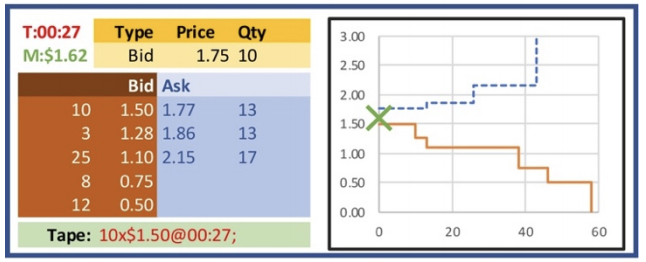
\includegraphics[width=0.8\textwidth]{LOB-Precross.png}
  \caption{A graphical representation of a Limit Order Book (LOB), reproduced from Cliff (2018)}
  }
\label{fig:lob}  
\end{figure}
\noindent
The left hand side of figure \ref{fig:lob} is a mockup of a graphical representation of BSE, whilst in its original form, is in a python dictionary data structure.
As seen in the figure, the bid book lists all the bid orders with their prices and the respective quantities available at that price as a key/value pair in descending order to represent all the outstanding orders from the buyers. Conversely, the ask book lists the price-quantity pair for all the ask orders in ascending order. In this order, the highest bid price is at the top of the bid book alongside the lowest ask price: the two prices are called the \textit{best bid} and the \textit{best ask} respectively. 
\\
\\
This graphical representation allows for easy feature extraction for some key elements that may not explicitly stated in the figure. 
\begin{itemize}
\item The \textit{Time Stamp} for the current time in the trading session, shown post-facing the "T" in the top left corner
\item The \textit{Bid-Ask Spread} which is the difference between the \textit{best ask} and the \textit{best bid}
\item The \textit{Midprice} is the arithmetic mean of the \textit{best ask} and the \textit{best bid}
\item The \textit{Tape} shows a record of all the executed trades and cancellations of orders
\item The \textit{Microprice} is a cross volume weighted average of the \textit{best ask} and \textit{best bid}, prefaced by the green "M" below the time stamp
\item The latest limit order sent to the exchange by a trader

\end{itemize}
\noindent
The \textit{midprice} and \textit{microprice} are values that are used to approximate the value of the asset and attempt to summarise the market. In this example snapshot figure \ref{fig:lob} the \textit{best ask} is \$1.77 and the \textit{best bid} is \$1.50 so the midprice is (\$1.77 +  \$1.50)/2 = \$1.66. The \textit{microprice} is a more intricate calculation because it is a cross volume weighted average:


\begin{equation}
\label{microprice}
\begin{split}
\frac{BestBidQty * BestAskPrice + BestAskQty*BestBidPrice}{ BestBidQty + BestAskQty}  = Microprice 
\end{split}
\end{equation}
\begin{equation}
\begin{split}
\frac{5*\$1.77 + 13*\$1.50}{5 + 18} = \$1.58
\end{split}
\end{equation}

\noindent
The right hand side of the figure represent the supply and demand curves curated from the ask and bid books respectively, where the orange line is the demand curve and the blue line is the supply curve.  Following the orange or blue step functions from left to right, at each step, the height represents the price and the width represents the available quantity at the price point. Lastly, the green cross represents the microprice.
\\
\\
A trade occurs when a bid offer's price is greater than the \textit{best ask} or when an ask offer's price is less than the \textit{best bid} on the LOB, this is known as \textit{crossing the spread}. This process is quantity invariant, that is if the latest order price crosses the spread but the requested quantity exceeds the quantity available at that price, all the quantities that are available are sold crossed price, and the unfulfilled quantities are then placed on the LOB as an outstanding order.
\\
\\
\noindent
As seen in the figure \ref{fig:lob}, the supply and demand curves do not cross, which therefore represents the fact that no trader is willing to trade at the current prices given in the exchange. The supply and demand curves not crossing means that the LOB is currently at equilibrium, as the best bid is not greater than the best ask.

\begin{figure}[H]
\centering{
  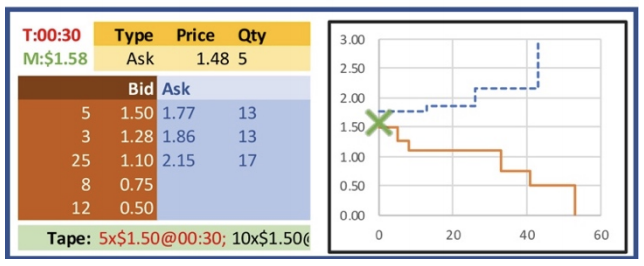
\includegraphics[width=0.8\textwidth]{LOB-Postcross.png}
  \caption{A graphical representation of a Limit Order Book (LOB), reproduced from Cliff (2018)}
  }
\label{fig:lob-post}  
\end{figure}
\noindent
The figure \ref{fig:lob-post} indicates that a new order has been placed to the exchange. Interestingly, this order crosses the spread because the ask price \$1.48 was less than the \textit{best bid} in figure \ref{fig:lob} so therefore a transaction occurs. Incidentally, the quantity requested was less than the quantity available at \$1.50 so the entire order is fulfilled, and the quantity remaining is updated from 10 to 5. For arguments sake, if the quantity requested was 20 rather than 5, all the quantities that are available at \$1.50 (10) would be used to fulfil the new order and then the LOB would have a new \textit{best bid} of \$1.48 with a qty of 10. 
\vspace{1cm}
\subsection{Proprietary trader's Objective}
\vspace{0.5cm}
The agents that are taking part in the 'gamification' of the trading session are sales traders. The aim of the sales trader is to maximise their consumer surplus relative to their client's order. As mentioned in the previous chapter, the sales trader does not hold a stock of their own, they trade on behalf of their \textit{client}, who provides them with a limit price that they cannot buy or sell above or below respectively. The goal of the sales trader is to maximise the difference between the limit price and the trade price, which is the consumer surplus. In the real world, the sales trader makes commission based on the consumer surplus and the client pockets the rest. 
\\
\\
The proprietary trader's objective is that to maximise their own capital buy buying and selling stocks for themselves. Whilst initially it may seem like the objective of the prop trader is different to the sales trader and therefore cant be compared, but the proprietary traders ability to maximise the difference between the price they buy and sell a stock at is analogous to a sales trader maximising the difference between its limit price and its trade price. This rephrasing of the problem allows this project to directly compare the traditional machine learning approaches to the prop trader developed in this project.

\section{Reinforcement Learning}

This project transforms the current Prop trader problem to a problem that is well suited to a DRL paradigm, which will be the main avenue of solutions this project explores, so it is paramount to provide the technical background for reinforcement learning, which is the basis of this project.

\subsection{Markov Decision Process}
Reinforcement Learning requires a fully observable environment 

% -----------------------------------------------------------------------------

\chapter{Project Execution}
\label{chap:execution}

{\bf A topic-specific chapter, of roughly $15$ pages} 
\vspace{1cm} 

\noindent
This chapter is intended to describe what you did: the goal is to explain
the main activity or activities, of any type, which constituted your work 
during the project.  The content is highly topic-specific, but for many 
projects it will make sense to split the chapter into two sections: one 
will discuss the design of something (e.g., some hardware or software, or 
an algorithm, or experiment), including any rationale or decisions made, 
and the other will discuss how this design was realised via some form of 
implementation.  

This is, of course, far from ideal for {\em many} project topics.  Some
situations which clearly require a different approach include:

\begin{itemize}
\item In a project where asymptotic analysis of some algorithm is the goal,
      there is no real ``design and implementation'' in a traditional sense
      even though the activity of analysis is clearly within the remit of
      this chapter.
\item In a project where analysis of some results is as major, or a more
      major goal than the implementation that produced them, it might be
      sensible to merge this chapter with the next one: the main activity 
      is such that discussion of the results cannot be viewed separately.
\end{itemize}

\noindent
Note that it is common to include evidence of ``best practice'' project 
management (e.g., use of version control, choice of programming language 
and so on).  Rather than simply a rote list, make sure any such content 
is useful and/or informative in some way: for example, if there was a 
decision to be made then explain the trade-offs and implications 
involved.

\section{Example Section}

This is an example section; 
the following content is auto-generated dummy text.
\lipsum

\subsection{Example Sub-section}

\begin{figure}[t]
\centering
foo
\caption{This is an example figure.}
\label{fig}
\end{figure}

\begin{table}[t]
\centering
\begin{tabular}{|cc|c|}
\hline
foo      & bar      & baz      \\
\hline
$0     $ & $0     $ & $0     $ \\
$1     $ & $1     $ & $1     $ \\
$\vdots$ & $\vdots$ & $\vdots$ \\
$9     $ & $9     $ & $9     $ \\
\hline
\end{tabular}
\caption{This is an example table.}
\label{tab}
\end{table}

\begin{algorithm}[t]
\For{$i=0$ {\bf upto} $n$}{
  $t_i \leftarrow 0$\;
}
\caption{This is an example algorithm.}
\label{alg}
\end{algorithm}

\begin{lstlisting}[float={t},caption={This is an example listing.},label={lst},language=C]
for( i = 0; i < n; i++ ) {
  t[ i ] = 0;
}
\end{lstlisting}

This is an example sub-section;
the following content is auto-generated dummy text.
Notice the examples in Figure~\ref{fig}, Table~\ref{tab}, Algorithm~\ref{alg}
and Listing~\ref{lst}.
\lipsum

\subsubsection{Example Sub-sub-section}

This is an example sub-sub-section;
the following content is auto-generated dummy text.
\lipsum

\paragraph{Example paragraph.}

This is an example paragraph; note the trailing full-stop in the title,
which is intended to ensure it does not run into the text.

% -----------------------------------------------------------------------------

\chapter{Critical Evaluation}
\label{chap:evaluation}

{\bf A topic-specific chapter, of roughly $15$ pages} 
\vspace{1cm} 

\noindent
This chapter is intended to evaluate what you did.  The content is highly 
topic-specific, but for many projects will have flavours of the following:

\begin{enumerate}
\item functional  testing, including analysis and explanation of failure 
      cases,
\item behavioural testing, often including analysis of any results that 
      draw some form of conclusion wrt. the aims and objectives,
      and
\item evaluation of options and decisions within the project, and/or a
      comparison with alternatives.
\end{enumerate}

\noindent
This chapter often acts to differentiate project quality: even if the work
completed is of a high technical quality, critical yet objective evaluation 
and comparison of the outcomes is crucial.  In essence, the reader wants to
learn something, so the worst examples amount to simple statements of fact 
(e.g., ``graph X shows the result is Y''); the best examples are analytical 
and exploratory (e.g., ``graph X shows the result is Y, which means Z; this 
contradicts [1], which may be because I use a different assumption'').  As 
such, both positive {\em and} negative outcomes are valid {\em if} presented 
in a suitable manner.

% -----------------------------------------------------------------------------

\chapter{Conclusion}
\label{chap:conclusion}

{\bf A compulsory chapter,     of roughly $5$ pages} 
\vspace{1cm} 

\noindent
The concluding chapter of a dissertation is often underutilised because it 
is too often left too close to the deadline: it is important to allocation
enough attention.  Ideally, the chapter will consist of three parts:

\begin{enumerate}
\item (Re)summarise the main contributions and achievements, in essence
      summing up the content.
\item Clearly state the current project status (e.g., ``X is working, Y 
      is not'') and evaluate what has been achieved with respect to the 
      initial aims and objectives (e.g., ``I completed aim X outlined 
      previously, the evidence for this is within Chapter Y'').  There 
      is no problem including aims which were not completed, but it is 
      important to evaluate and/or justify why this is the case.
\item Outline any open problems or future plans.  Rather than treat this
      only as an exercise in what you {\em could} have done given more 
      time, try to focus on any unexplored options or interesting outcomes
      (e.g., ``my experiment for X gave counter-intuitive results, this 
      could be because Y and would form an interesting area for further 
      study'' or ``users found feature Z of my software difficult to use,
      which is obvious in hindsight but not during at design stage; to 
      resolve this, I could clearly apply the technique of Smith [7]'').
\end{enumerate}

% =============================================================================

% Finally, after the main matter, the back matter is specified.  This is
% typically populated with just the bibliography.  LaTeX deals with these
% in one of two ways, namely
%
% - inline, which roughly means the author specifies entries using the 
%   \bibitem macro and typesets them manually, or
% - using BiBTeX, which means entries are contained in a separate file
%   (which is essentially a databased) then imported; this is the 
%   approach used below, with the databased being dissertation.bib.
%
% Either way, the each entry has a key (or identifier) which can be used
% in the main matter to cite it, e.g., \cite{X}, \cite[Chapter 2}{Y}.

\backmatter

\bibliography{dissertation}


% -----------------------------------------------------------------------------

% The dissertation concludes with a set of (optional) appendicies; these are 
% the same as chapters in a sense, but once signaled as being appendicies via
% the associated macro, LaTeX manages them appropriatly.

\appendix

\chapter{An Example Appendix}
\label{appx:example}

Content which is not central to, but may enhance the dissertation can be 
included in one or more appendices; examples include, but are not limited
to

\begin{itemize}
\item lengthy mathematical proofs, numerical or graphical results which 
      are summarised in the main body,
\item sample or example calculations, 
      and
\item results of user studies or questionnaires.
\end{itemize}

\noindent
Note that in line with most research conferences, the marking panel is not
obliged to read such appendices.

% =============================================================================

\end{document}
